\documentclass{article}
\usepackage[utf8]{inputenc}
\usepackage[french]{babel}

\textwidth 16.2cm \textheight 23cm \topmargin -0.6cm
\oddsidemargin 0.31cm \evensidemargin -0.91cm

\usepackage{amsmath}
\usepackage{amsfonts}
\usepackage{amsbsy}
\usepackage{amssymb}
\usepackage{algorithme}
\usepackage{graphicx}
\usepackage{psfrag}
\usepackage{epsfig}
\usepackage{multicol}
\usepackage{cite}
\usepackage{color}
\usepackage{dsfont}
\usepackage[center]{caption}
\usepackage{listings} 
\usepackage{xcolor} 
\usepackage{textcomp} 
%\usepackage{enumitem}
\usepackage{hyperref}

\hypersetup{
    bookmarks=true,         % show bookmarks bar?
    unicode=false,          % non-Latin characters in Acrobat’s bookmarks
    pdftoolbar=true,        % show Acrobat’s toolbar?
    pdfmenubar=true,        % show Acrobat’s menu?
    pdffitwindow=false,     % window fit to page when opened
    pdfstartview={FitH},    % fits the width of the page to the window
    pdftitle={My title},    % title
    pdfauthor={Author},     % author
    pdfsubject={Subject},   % subject of the document
    pdfcreator={Creator},   % creator of the document
    pdfproducer={Producer}, % producer of the document
    pdfkeywords={keyword1} {key2} {key3}, % list of keywords
    pdfnewwindow=true,      % links in new window
    colorlinks=true,       % false: boxed links; true: colored links
    linkcolor=red,          % color of internal links (change box color with linkbordercolor)
    citecolor=blue,        % color of links to bibliography
    filecolor=magenta,      % color of file links
    urlcolor=cyan,           % color of external links
	pdfborder	= {0 0 0}
}

\newcommand {\defeq}    {\stackrel{\rm def}{=}}

\DeclareMathOperator{\Span} {{Span}}
\DeclareMathOperator{\gap} {{gap}}
\DeclareMathOperator{\ddiv} {{div}}
\DeclareMathOperator{\argsup} {{argsup}}
\DeclareMathOperator{\argmin} {{argmin}}
\DeclareMathOperator{\dom} {{dom}}
\DeclareMathOperator{\epi} {{epi}}

\newtheorem{thm}{Theorem}
\newtheorem{prop}{Proposition}
\newtheorem{lemma}{Lemma}
\newtheorem{defn}{Definition}
\newtheorem{cor}{Corollary}
\newtheorem{model}{Model}
\newtheorem{rmk}{Remarque}
\newtheorem{ans}{Answer}
\newtheorem{ass}{Assumption}
\newtheorem{algo}{Algorithme}

\newcommand{\G}{\mathcal{G}}
\newcommand{\lab}{\text{label}}

\def\endproof{\hfill $\Box$\newline\newline}
\def\proof{\par\noindent{\it Proof}. \ignorespaces}

\title{Projet de département}
\author{Marie Rozand, Raphael Sivera, Yohann Salaun}
\date{\today}

\parindent=0pt
\begin{document}
\maketitle

\section{Coupes de graphes}

Les méthodes de coupes de graphe permettent de résoudre des problèmes de classification binaire. Généralement coûteuse en temps et en mémoire, ce type de méthode nous servira en fin d'algorithme pour affiner et régulariser la détection des \textit{TODO} dans les images. Cette section présente brièvement la théorie des coupes de graphes et son application à notre projet. De nombreuses informations complémentaires concernant les coupes de graphes peuvent être trouvées dans \cite{bib:GC04, bib:GC05}.		

\subsection{Théorie}

On considère ici une image que l'on veut segmenter en deux parties. Le problème consiste donc à attribuer à chacun des points de l'image un label correspondant à l'une ou l'autre des classes de segmentation.

\subsubsection{Formulation énergétique}

Ce problème de classification peut s'écrire sous la forme d'une minimisation d'énergie dont la valeur dépend de l'affectation de chacun des points. Les points ont tendances à appartenir à l'une des classes lorsque d'une part leurs paramètres intrinsèques les y amènent (intensité, gradient local, ...) mais également lorsque leurs voisins y appartiennent ou non (connexité des parties à segmenter). Cette énergie est alors constituée de 2 termes:
\begin{itemize}
	\item[$\bullet$]\textbf{Terme d'attache aux données :} fonction d'un point et de ses paramètres pour favoriser son attache à l'un ou l'autre des labels de classification.
	\item[$\bullet$]\textbf{Terme de régularisation :} fonction de plusieurs points jugés \textit{voisins} (c'est à dire que leurs affectations respectives dépendent l'une de l'autre).
\end{itemize}
L'énergie s'écrit alors sous la forme:
\[
	E_{TOTAL} = \sum_{\lab \in \{s,t\}} \sum_{p \in \mathcal{G}} E_{DATA}(\lab, p) + \lambda \sum _{p,q \in \mathcal{G} \text{ voisins}} E_{SMOOTH}(p,q)
\]
où $\lambda$ est appelé terme de régularité et permet de modifier l'importance du rapport attache-aux-données/régularité.\\

\subsubsection{Forme des graphes}

Il est également possible de modéliser le problème sous la forme d'un graphe $\G$. Ce graphe contient l'ensemble des points à classifier représentés sous la forme de ses sommets auxquels on ajoute 2 sommets particuliers généralement notés $s$ (pour \textit{source}) et $t$ (pour \textit{target}). Les points sont tous reliés par des arêtes à $s$ et $t$ qui représentent les 2 \textit{labels} de classification du problème. Par ailleurs, on relie les points entre eux lorsque l'affectation de l'un est fonction de l'affectation de l'autre.\\
On obtient alors un graphe de la forme : 
\begin{figure}
	\begin{center}
		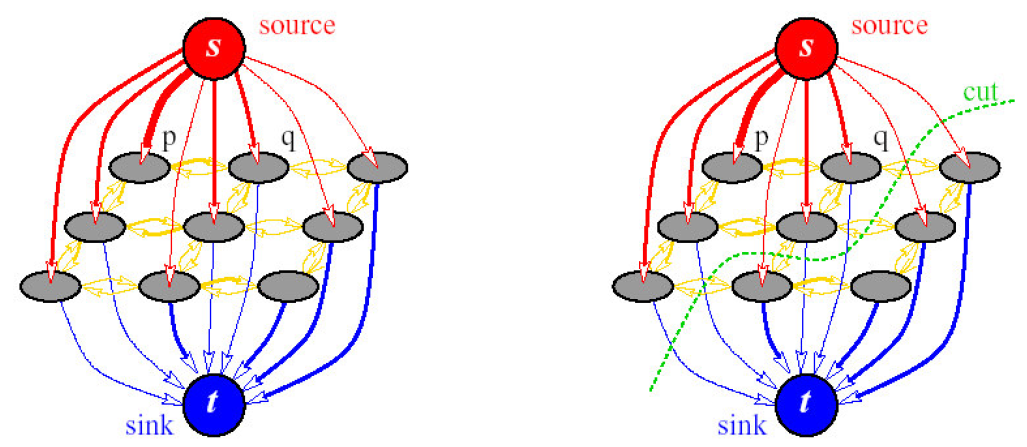
\includegraphics[width=0.8\textwidth]{Images/GC/graphcut.png} 
	\end{center}
	\caption{Forme classique d'un graphe utilisable dans les méthodes de coupes de graphe. A gauche, le graphe avec les 2 noeuds principaux $s$ et $t$. A droite, un exemple de coupe de graphe. Les arêtes en gras relient les sommets aux labels définis par la coupe.}
	\label{fig:GC_graphe}
\end{figure}

\subsubsection{Coupes minimales}

On dit que $\mathcal{C}$ est une \textbf{coupe} du graphe $\G$ si elle sépare $\G$ en deux ensembles connexes disjoints $\mathcal{S},\mathcal{T}$ tels que  
$s \in \mathcal{S}$ et $t \in \mathcal{T}$.\\
On peut alors définir la \textbf{capacité} de la coupe $\mathcal{C}$ par :
\[
	c(\mathcal{C}) = \sum_{(u,v) \in \mathcal{S} \times \mathcal{T}} c_{uv}
\]
où $c_{uv}$ est le poids assigné à l'arête $[u,v]$.\\
Une coupe de $\G$ est alors minimale lorsqu'il n'existe pas d'autres coupes dont la capacité est inférieure strictement. Cependant, il n'y a en général pas unicité de la coupe minimale. De nombreux algorithme permettent de calculer la coupe minimale d'un graphe via le calcul de son équivalent, le \textbf{flot maximum}. En effet, le flot maximum est facilement calculable avec des algorithmes gloutons par exemple. \\
On cherche donc à se ramener au problème de calcul de coupe minimale en affectant aux arêtes les poids suivants:
\begin{itemize}
	\item[$\bullet$] Un terme d'attache aux données, lorsque l'arête relie un sommet quelconque à $t$ ou $s$: $E_{DATA}(\lab, p)$
	\item[$\bullet$] Un terme de régularité, lorsque l'arête relie deux sommets voisins $p$ et $q$: $E_{SMOOTH}(p,q)$
\end{itemize}
On rend alors équivalents la minimisation de l'énergie $E_{TOTAL}$ et la recherche de la coupe minimale de $\G$.\\
Le calcul de la coupe minimale du graphe $\G$ ainsi construit permet de minimiser l'énergie et donc de résoudre le problème de classification.

\subsection{Application dans le cadre de la détection de TODO}

Pour appliquer des méthodes de coupes de graph au sujet qui nous intéresse, il s'agit alors de définir les fonctions d'attaches aux données et de régularisation d'une part et de construire un graphe $\G$ représentatif du problème d'autre part.

\subsubsection{Construction du graphe}

A chaque voxel de l'image on associe un sommet $p$ du graphe. On ajoute également $s_{IN}$ pour le label \textit{interieur} et $s_{OUT}$ pour le label \textit{exterieur}. Les sommets étant définis, il s'agit alors de les relier entre eux avec des arêtes correspondants à la réalité du problème.\\
On relie donc chaque sommets $p$ à $s_{IN}$ et $s_{OUT}$. En remarquant par ailleurs que la complexité de la minimalisation de la coupe dépend du nombre d'arêtes dans le graphe, on se contente d'appliquer un modèle de 6-connexité pour les arêtes reliant 2 sommets $p$ voisins. C'est à dire que l'affectation chaque voxel ne dépend que de l'affectation de ses 6 voisins les plus proches, comme le montre la figure \textit{TODO !!!}

\subsubsection{Energies}

L'énergie d'attache aux données se calcule à partir des probabilités définies dans les parties précédentes. Celles-ci permettent d'avoir une information grossière sur la forme de l'objet à détecter. On suppose que cette probabilité est relativement proche de la réalité et on définit ainsi l'énergie d'attache aux données par :
\begin{center}
\begin{itemize}
	\item[$\bullet$] $E_{DATA}(s_{IN}, p) = f(\mathbb{P}(p \in s_{IN}))$
	\item[$\bullet$] $E_{DATA}(s_{OUT}, p) =f( \mathbb{P}(p \in s_{OUT}))$
\end{itemize}
\end{center}
$f$ peut être la fonction \textit{valeur absolue} ou \textit{carrée} par exemple.
\\
\\
L'énergie de régularisation est nulle lorsque les labels des 2 voxels voisins sont les mêmes. Dans le cas contraire, elle dépend de deux paramètres:
\begin{itemize}
	\item[$\bullet$] la différence d'intensité entre les 2 voxels doit être suffisament importante. En effet, 2 voxels voisins d'intensité similaire appartiennent certainement au même objet. La réciproque n'est par contre pas vérifiée.
	\item[$\bullet$] la localisation de leur barycentre. En effet, celui-ci est sensé appartenir à la frontière séparant les 2 objets.
\end{itemize}
En suivant les conseils de \cite{bib:seg}, nous avons utilisé les énergies suivantes:
\begin{itemize}
	\item[$\bullet$] pour la différence d'intensité: $E_{SMOOTH 1} \varpropto e^{-\frac{\Delta I^2}{2\sigma^2}}$ où $\Delta I$ est l'écart d'intensité et $\sigma$ est le paramètre de pénalisation.
	\item[$\bullet$] pour la localisation du barycentre: $E_{SMOOTH 2} \varpropto  \frac{d^2}{2\sigma^2}$ où $d$ est la distance du barycentre à la frontière.
\end{itemize}
Les fonctions utilisées peuvent être quelconques à partir du moment où elles vérifient la condition de \textbf{régularité}:
\begin{equation*}
\forall i, j \{VOXEL\}, \ \ \forall l_1, l_2 \in \{LABEL\}\ \  E(i\rightarrow l_1, j\rightarrow l_1) + E(i\rightarrow l_2, j\rightarrow l_2) \leq E(i\rightarrow l_1, j\rightarrow l_2) + E(i\rightarrow l_2, j\rightarrow l_1)
\end{equation*}
Cette condition est évidemment vérifiée dans le cas précédent puisque l'égalité des labels entraine la nullité du terme de régularité et que les autres termes sont positifs ou nuls.

\bibliographystyle{plain} %Style of Bibliography: plain / apalike / amsalpha / ...
\bibliography{literature} %You need a file 'literature.bib' for this.

\end{document}
